\section{Simulations}
\subsection{1 DOF Vertical Hopper with Open-loop Control\cite{Cham2002}}
\subsubsection*{System Setup}
\begin{itemize}
\item body mass $m=1$ with massless leg.
\item $l=1$
\item $\omega_n = 30$
\item $\xi = 0.15$ (or equivalently, $kp = 900, kd = 9$)
\item static initial condition, COM height = 0.3
\item open-loop force control:
\begin{align*}
 f_n(t)=\begin{cases}
    f_n\in \mathbb{C}, & \text{if $t \in t_{on}$}.\\
    0, & \text{otherwise}.
  \end{cases}
\end{align*}
  \item $t_{on}$: The duration of actuator activation, starts when the spring reaches the maximum compression, ends when the contact point leave the ground.
  \begin{figure}[H]
  \centering
  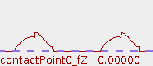
\includegraphics[scale =1.5]{GRF_openloop.pdf} 
  \caption{Ground reaction force when $f_n = 10$}
%  \label{fig.verticalHopper1DOF}
  \end{figure}
  
\end{itemize}
\begin{figure}[H]
\centering
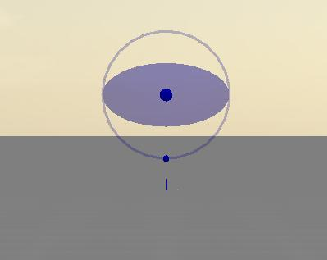
\includegraphics[scale = 0.7]{verticalHopper1DOF.pdf} 
\caption{The vertical hopper, the blue dot at the bottom is the contact point of the massless leg.}
\label{fig.verticalHopper1DOF}
\end{figure}

\begin{figure}[H] 
\centering
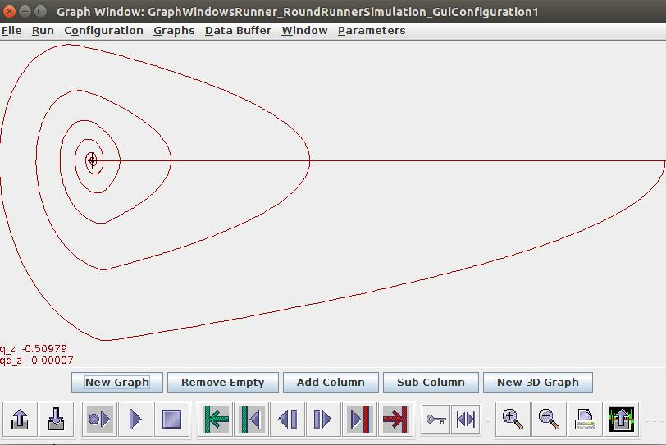
\includegraphics[scale = 0.7]{f1_stable_T0.pdf} 
\caption{Phase portrait (stable spiral) of $f = 1$, period $0$ sec}
%\label{fig.verticalHopper1DOF}
\end{figure}
\begin{figure}[H] 
\centering
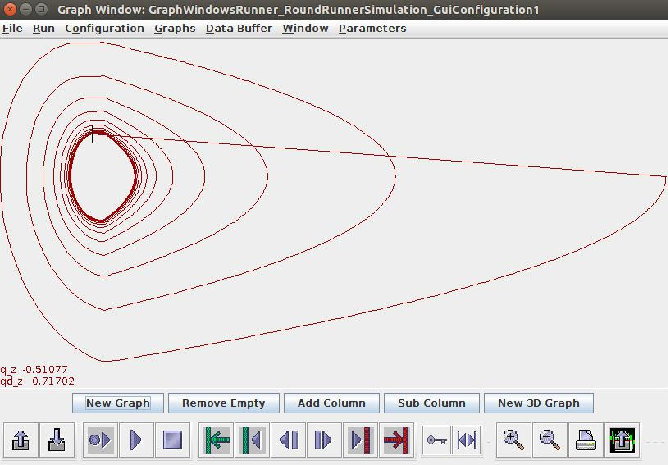
\includegraphics[scale = 0.7]{f10_stable_T0270.pdf} 
\caption{Phase portrait (stable limit cycle) of $f = 10$, period $0.27$sec, (closer to the damped natural period $\approxeq 0.3295$ sec)}
%\label{fig.verticalHopper1DOF}
\end{figure}

\begin{figure}[H]
\centering
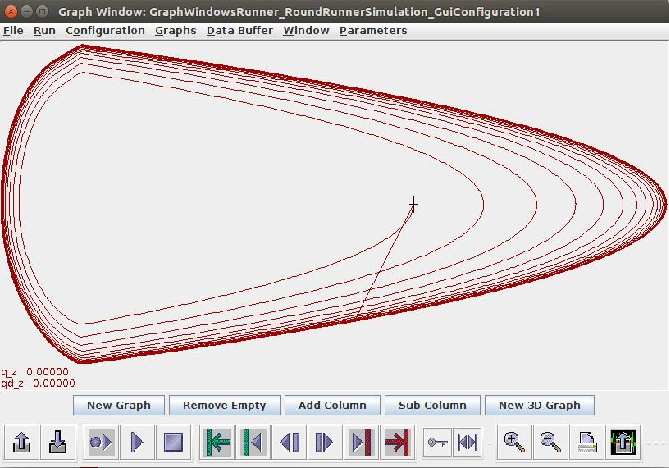
\includegraphics[scale = 0.7]{f50_stable_T0859.pdf} 
\caption{Phase portrait (stable limit cycle) of $f = 50$, period $0.859$ sec}
%\label{fig.verticalHopper1DOF}
\end{figure}

\begin{figure}[H]
\centering
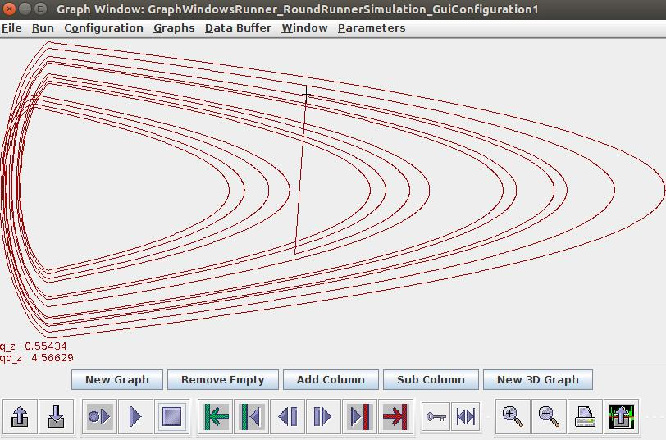
\includegraphics[scale = 0.8]{f100_unstable.pdf} 
\caption{Phase portrait of $f = 100$, no stable limit cycle evolved (might be bifurcation).}
%\label{fig.verticalHopper1DOF}
\end{figure}

\pagebreak